\documentclass[11pt,a4paper]{article}
\usepackage{amsmath}
\usepackage{amsfonts}
\usepackage{amssymb}
\usepackage{graphicx}
\usepackage[margin=1in]{geometry}
\usepackage{hyperref}
\usepackage{listings}
\usepackage{xcolor}

\title{Mesoscopic Model: Computational Framework for Dynamics Study}
\author{Research Project}
\date{\today}

\begin{document}

\maketitle

\tableofcontents
\newpage

\section{Background}

\subsection{Ising Models}

The Ising model is a fundamental statistical mechanical model that describes the behavior of magnetic systems. For a two-dimensional square lattice with nearest-neighbor interactions, the Hamiltonian is given by:

\begin{equation}
H = -J \sum_{\langle i,j \rangle} s_i s_j - h \sum_i s_i
\end{equation}

where $s_i \in \{-1, +1\}$ are the spin variables, $J$ is the coupling strength, $h$ is the external magnetic field, and $\langle i,j \rangle$ denotes nearest-neighbor pairs.

\subsubsection{Critical Temperature}

The critical temperature $T_c$ is a fundamental parameter that determines the phase transition between ordered and disordered phases. We experimentally use $T_c = 1.0$ and $T_c = 4.0$.

\begin{equation}
T_c = \frac{2J}{k_B \ln(1 + \sqrt{2})} \approx \frac{2.269J}{k_B}
\end{equation}

where $k_B$ is the Boltzmann constant. This critical temperature separates two distinct phases:

\begin{itemize}
    \item \textbf{High temperature regime} ($T > T_c$): The system is in a \textit{disordered phase} where spins are randomly oriented, resulting in zero net magnetization. The system exhibits thermal fluctuations and short-range correlations.
    
    \item \textbf{Low temperature regime} ($T < T_c$): The system is in an \textit{ordered phase} where spins tend to align, leading to non-zero magnetization. The system exhibits long-range order and reduced thermal fluctuations.
    
    \item \textbf{Critical region} ($T \approx T_c$): The system undergoes a phase transition with critical phenomena, including diverging correlation lengths and power-law scaling behavior.
\end{itemize}

The temperature ratio $T/T_c$ is a key parameter that determines the physical regime of the system. In our simulations, we often work in the high-temperature regime where $T/T_c > 1$, corresponding to the disordered phase.

\subsubsection{Units and Normalization}

In our computational framework, we use dimensionless units where the Boltzmann constant $k_B = 1$ and the coupling strength $J = 1$. This normalization simplifies the calculations while preserving the essential physics. The temperature $T$ is therefore dimensionless, and the critical temperature becomes:

\begin{equation}
T_c = \frac{2}{\ln(1 + \sqrt{2})} \approx 2.269
\end{equation}

This approach is common in computational statistical physics as it eliminates the need to track physical units while maintaining the correct scaling relationships between temperature, energy, and other thermodynamic quantities.

In this normalization, the inverse temperature $\beta = 1/T$ is directly computed from the dimensionless temperature $T$. For example, with $T = 6.808$, we have $\beta = 1/6.808 \approx 0.147$, which represents the strength of thermal fluctuations in the system.

\section{PDE}

\subsection{Hydrodynamic Limit for Glauber-Kac}

\begin{equation}\label{eq:nonlocal}
    \partial_t m(t,\mathbf{x}) \;=\; -\,m(t,\mathbf{x})\;+\;\tanh\!\Big(\beta\, (J_\gamma * m)(t,\mathbf{x}) + \beta h\Big), \qquad m(0,\mathbf{x})=m_0(\mathbf{x}),
    \end{equation}
where $(J_\gamma * m)(\mathbf{x})=\int_{\bbT^d}J_\gamma(\mathbf{x}-\mathbf{y})m(\mathbf{y})\,d\mathbf{y}$ is a Kac-type kernel, where we use a Gaussian kernel as an example.  

\begin{equation}
    J_\gamma(\mathbf{x}) = \frac{1}{(2\pi\gamma^2)^{d/2}} \exp\left(-\frac{|\mathbf{x}|^2}{2\gamma^2}\right)
\end{equation}


\section{Numerical Results}
\subsection{Experimental Settings}

\subsubsection{Parameter Configuration}

Our computational experiments are designed to systematically explore the parameter space of the Ising model and its mesoscopic approximations. The base configuration uses:

\begin{itemize}
    \item \textbf{Coupling strength}: $J = 1.0$ (dimensionless units)
    \item \textbf{Critical temperature}: $T_c = 2.27$ (for 2D square lattice)
    \item \textbf{Lattice size}: $L = 1024$ with coarse-graining to $M = 128$
    \item \textbf{Block size}: $B = 8$ (coarse-graining ratio $L/M = 8$)
    \item \textbf{Spatial resolution}: $\delta = 1/M = 0.007812$
\end{itemize}

\subsubsection{Temperature Regimes}

We investigate two distinct temperature regimes:

\begin{enumerate}
    \item \textbf{Low temperature} ($T = 1.0$): Below critical temperature, corresponding to the ordered phase where $T/T_c \approx 0.44$
    \item \textbf{High temperature} ($T = 3.0$): Above critical temperature, corresponding to the disordered phase where $T/T_c \approx 1.32$
\end{enumerate}

\subsubsection{External Field Variations}

The external magnetic field $h$ is varied across four values to study its effect on the system dynamics:

\begin{itemize}
    \item $h = 0.0$ (no external field)
    \item $h = 0.5$ (weak external field)
    \item $h = 1.0$ (moderate external field)
    \item $h = 2.0$ (strong external field)
\end{itemize}

\subsubsection{Kernel Range Studies}

To investigate the role of interaction range in nonlocal dynamics, we vary the kernel domain size:

\begin{itemize}
    \item \textbf{Local interactions}: $\gamma = \delta$ (nearest-neighbor only)
    \item \textbf{Short-range nonlocal}: $\gamma = 2\delta$ (extended local interactions)
    \item \textbf{Medium-range nonlocal}: $\gamma = 4\delta$ (moderate nonlocal interactions)
\end{itemize}

This systematic variation allows us to study the transition from local to nonlocal behavior and its impact on pattern formation and dynamics.

This computational framework will provide insights into:

\begin{itemize}
    \item The relationship between microscopic and macroscopic dynamics
    \item The validity of continuum approximations
    \item The role of nonlocal interactions in pattern formation
    \item Machine learning approaches for complex dynamics
\end{itemize}

\subsection{Data v.s. PDE Solutions}

% with epsilon = 0.015625

\begin{figure}[!h]
    \centering
    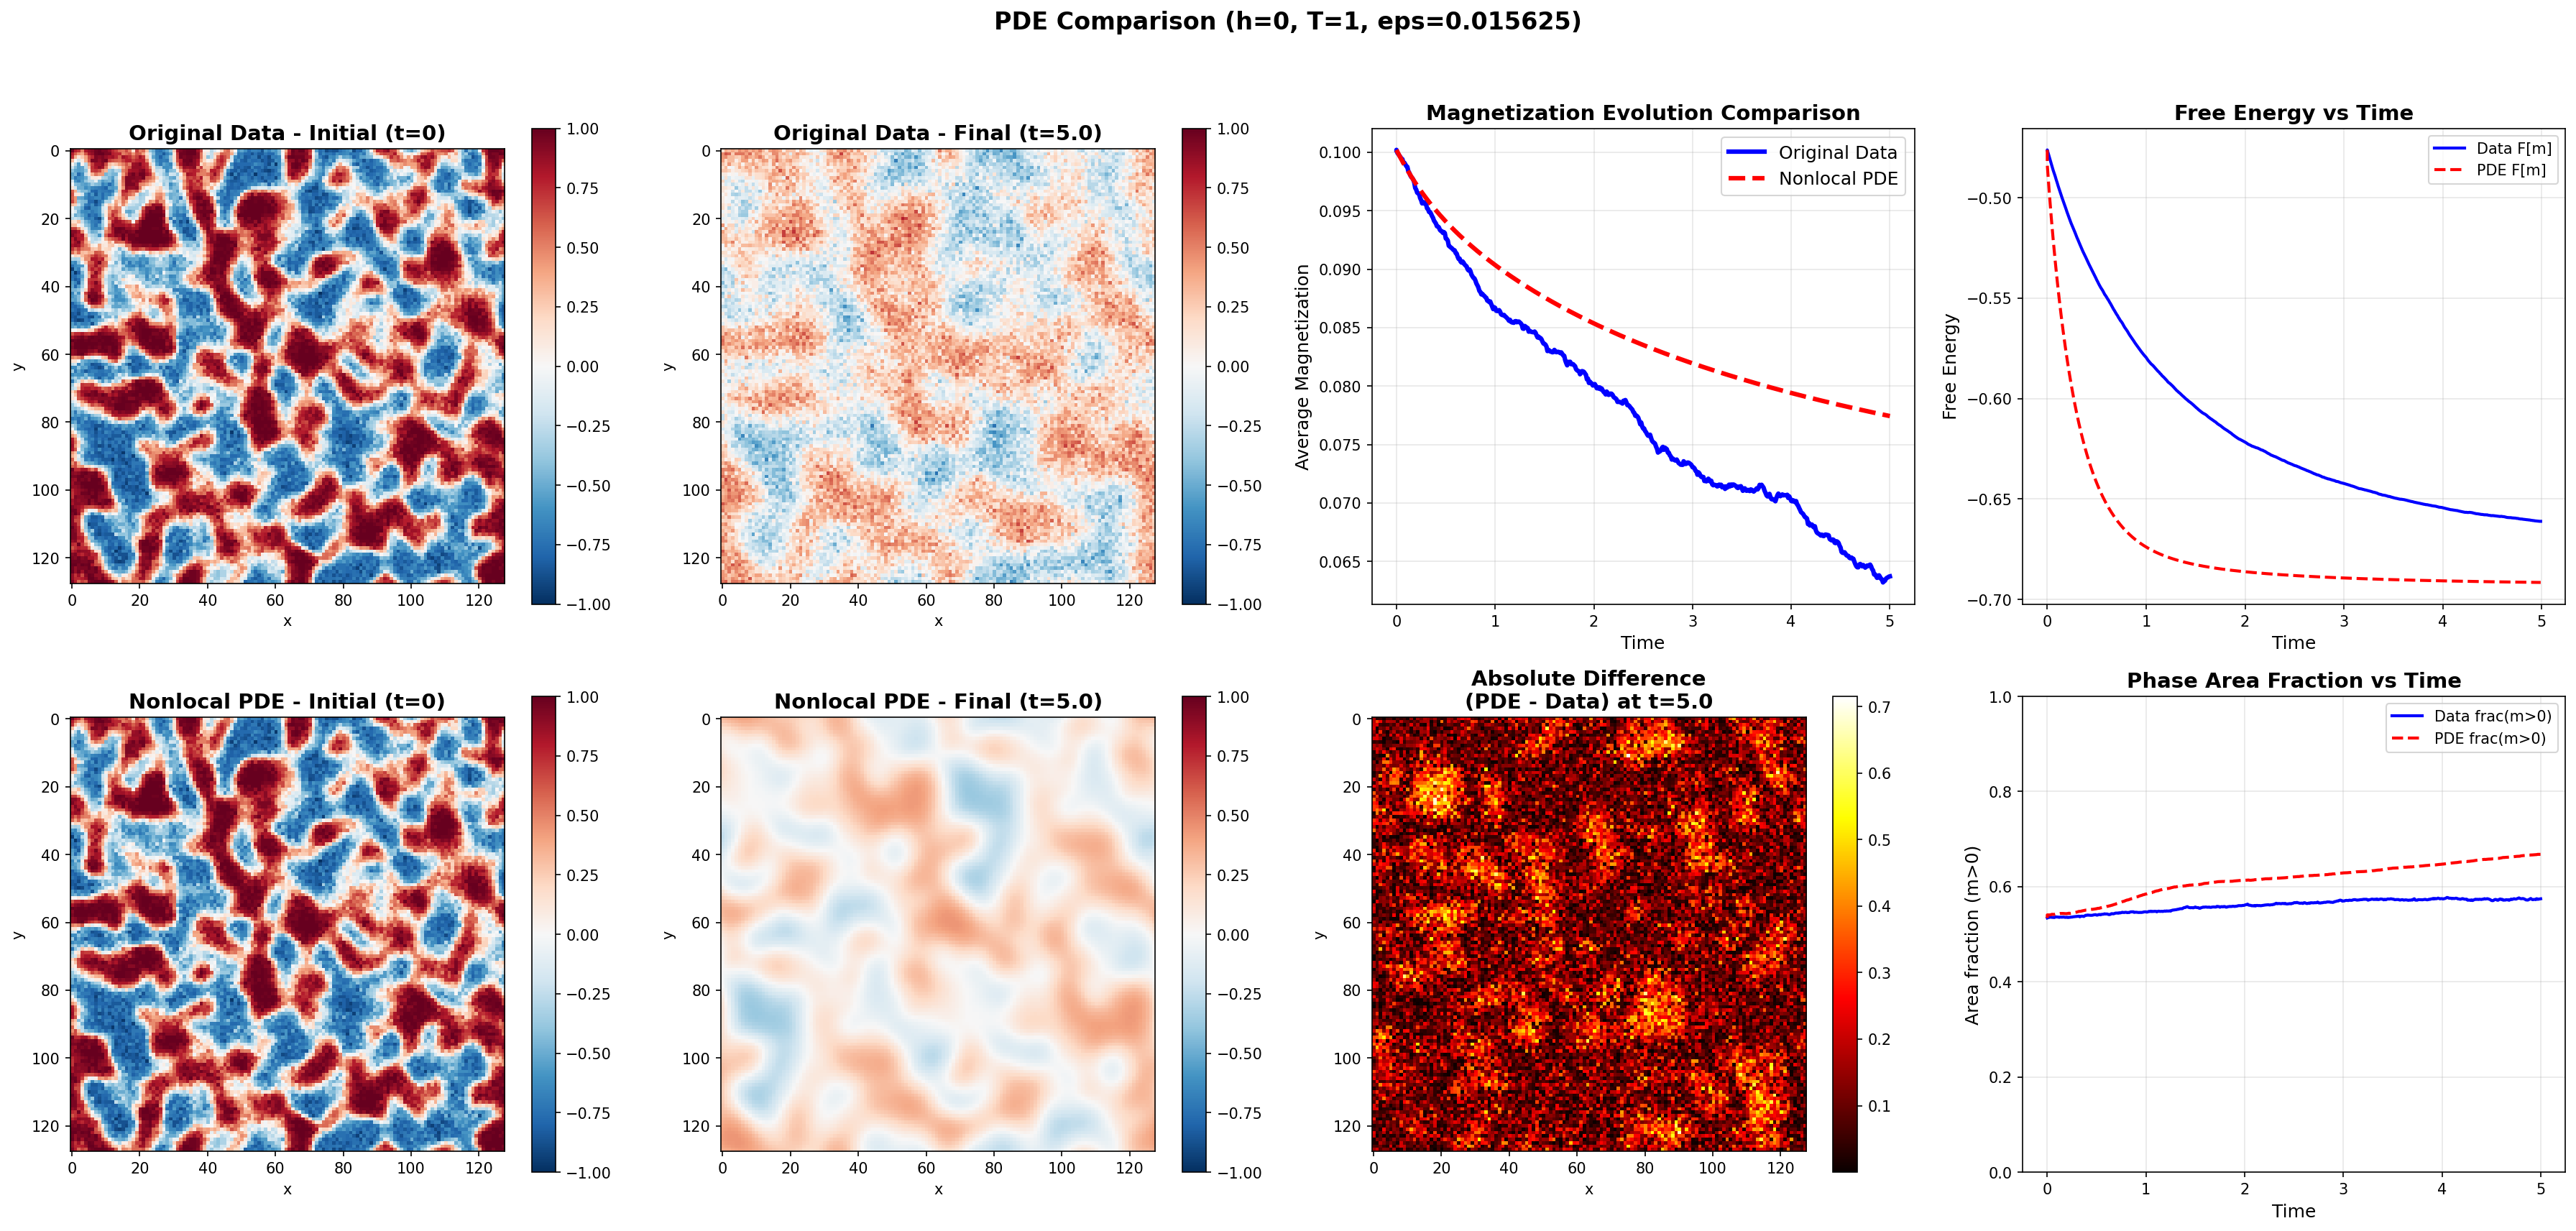
\includegraphics[width=1.0\textwidth]{fig/pde_comparison_h0_T1_eps0.015625.png}
    \caption{Comparison of original data and PDE solutions for $h=0$, $T=1$, $\epsilon=0.015625$.}
\end{figure}


\begin{figure}[!h]
    \centering
    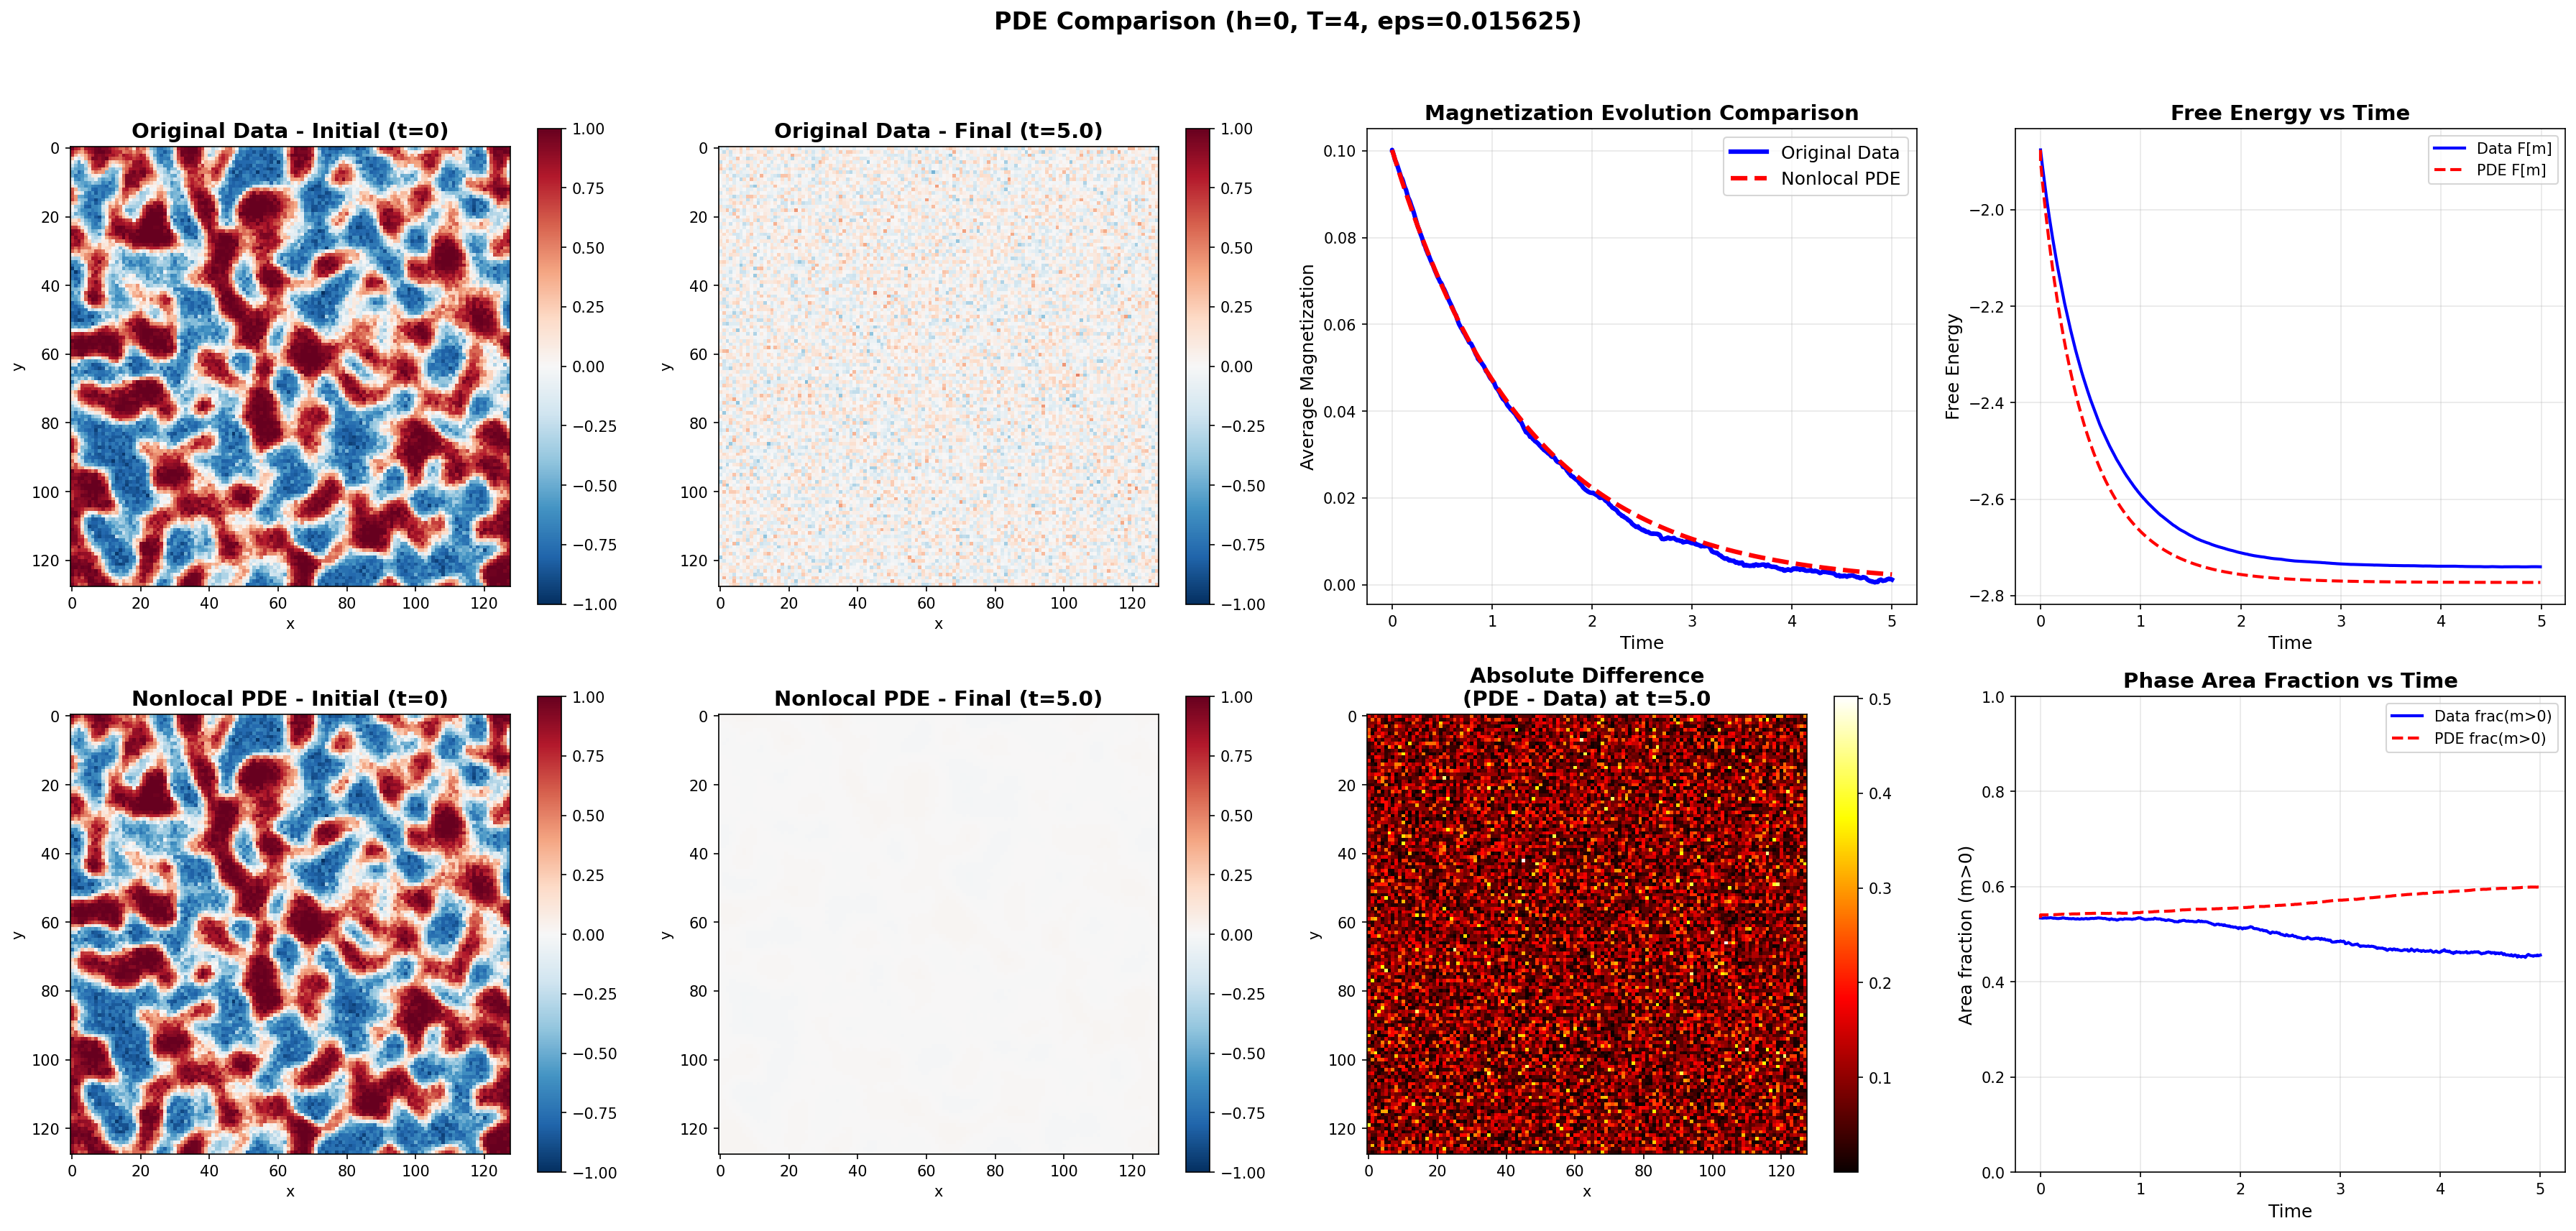
\includegraphics[width=1.0\textwidth]{fig/pde_comparison_h0_T4_eps0.015625.png}
    \caption{Comparison of original data and PDE solutions for $h=0$, $T=4$, $\epsilon=0.015625$.}
\end{figure}


\begin{figure}[!h]
    \centering
    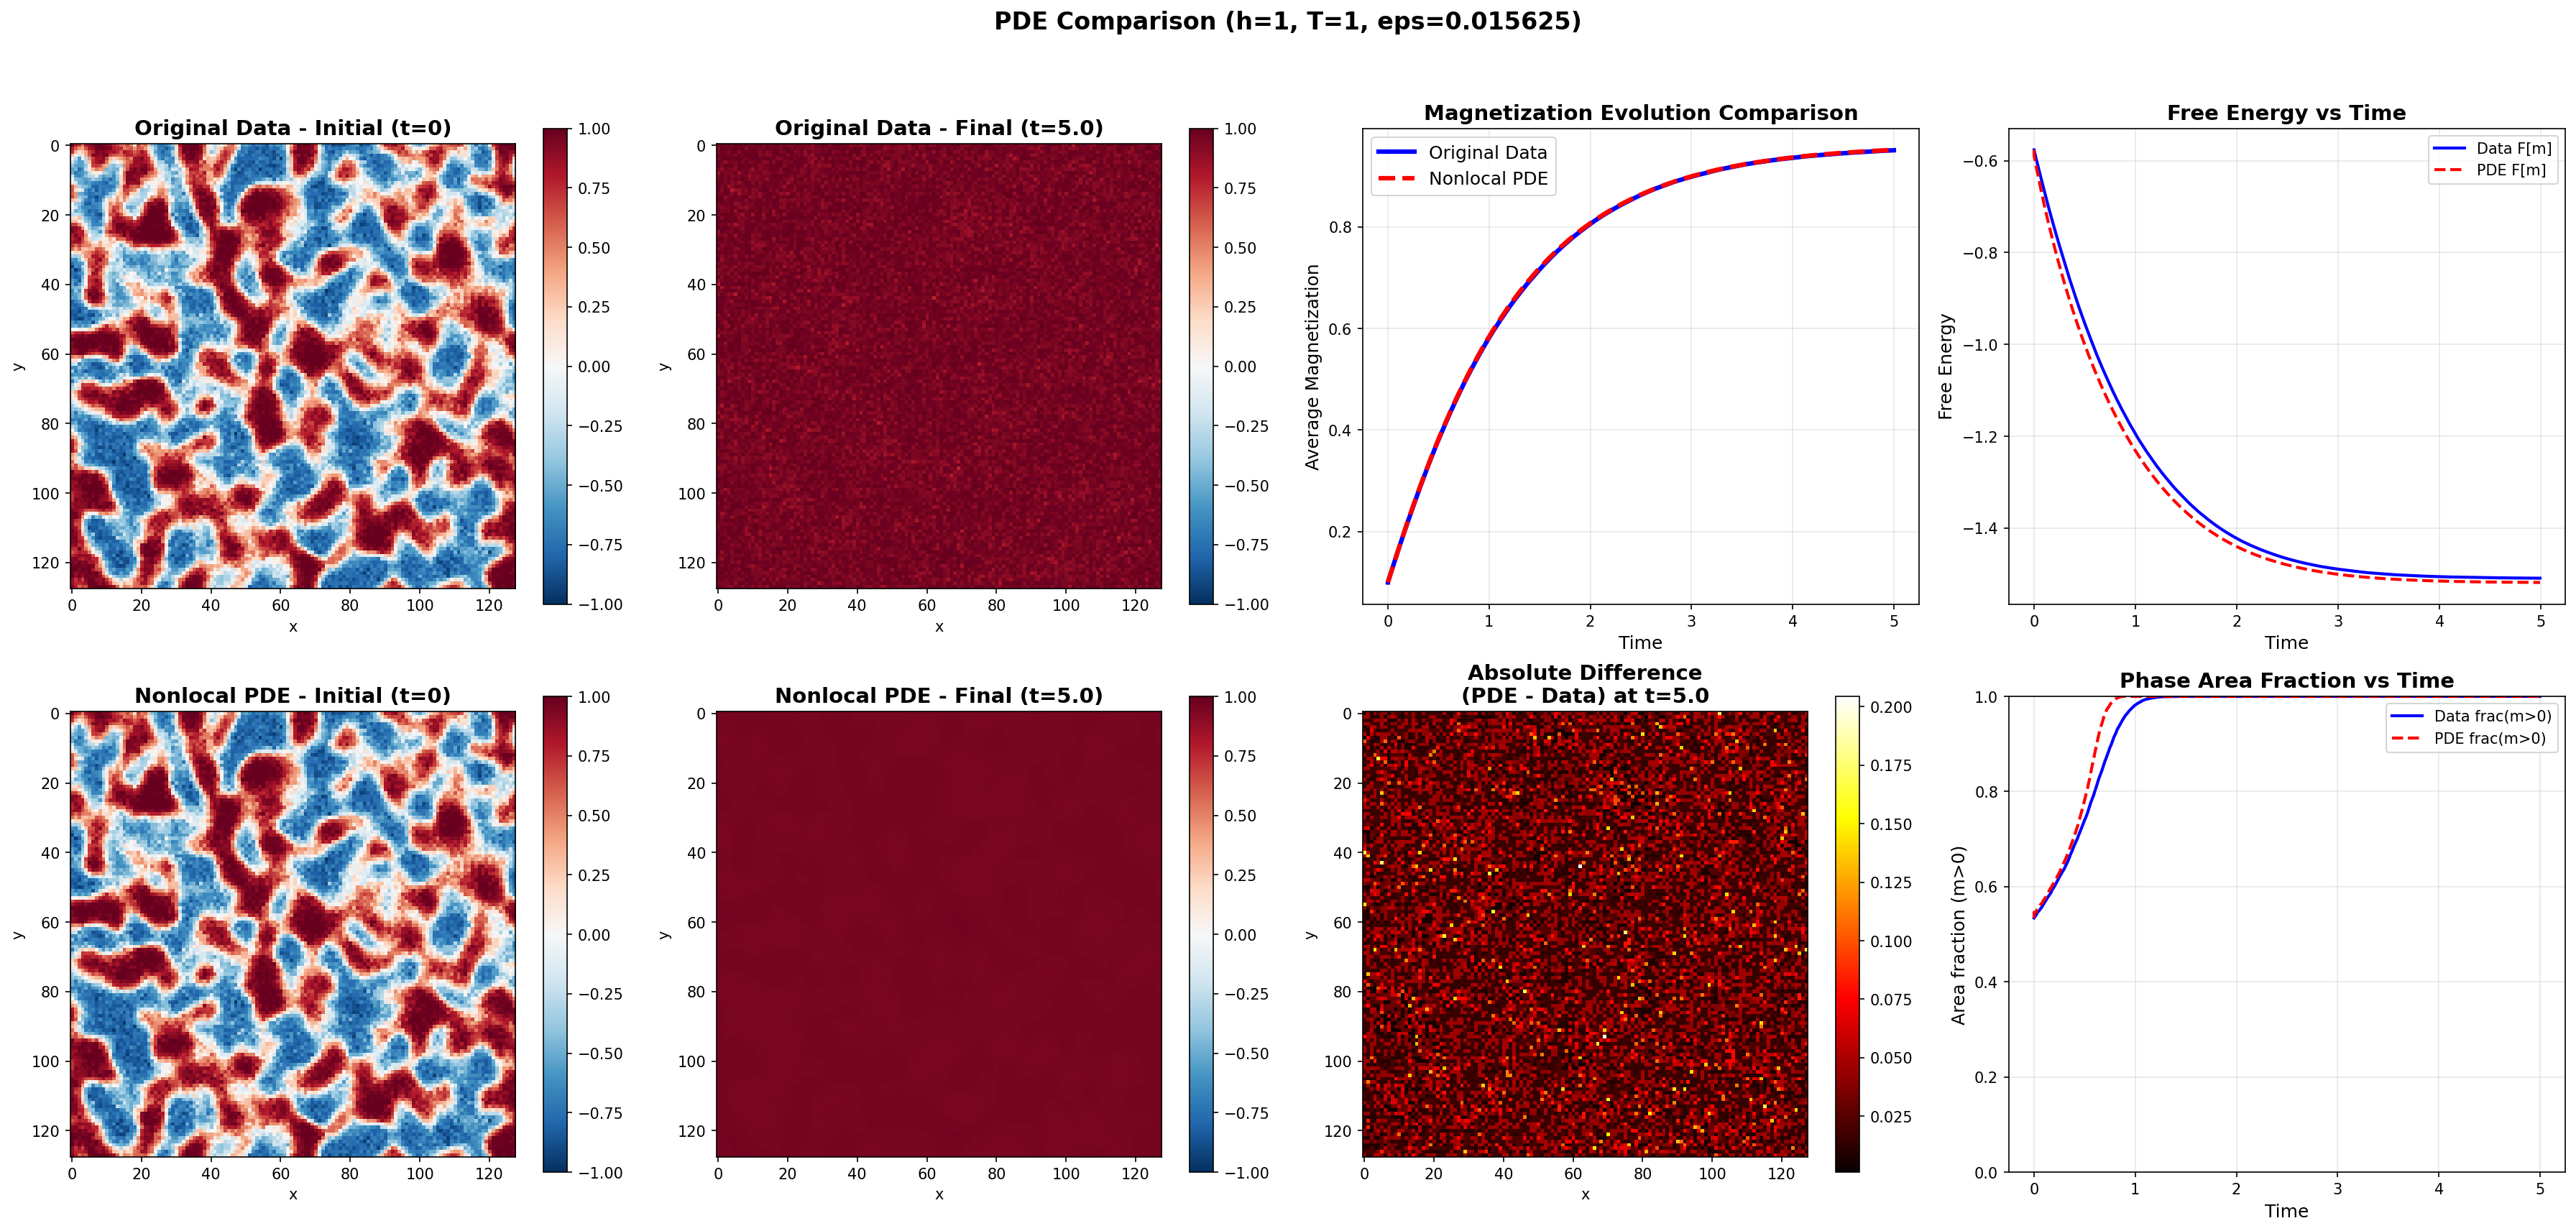
\includegraphics[width=1.0\textwidth]{fig/pde_comparison_h1_T1_eps0.015625.png}
    \caption{Comparison of original data and PDE solutions for $h=1$, $T=1$, $\epsilon=0.015625$.}
\end{figure}


\begin{figure}[!h]
    \centering
    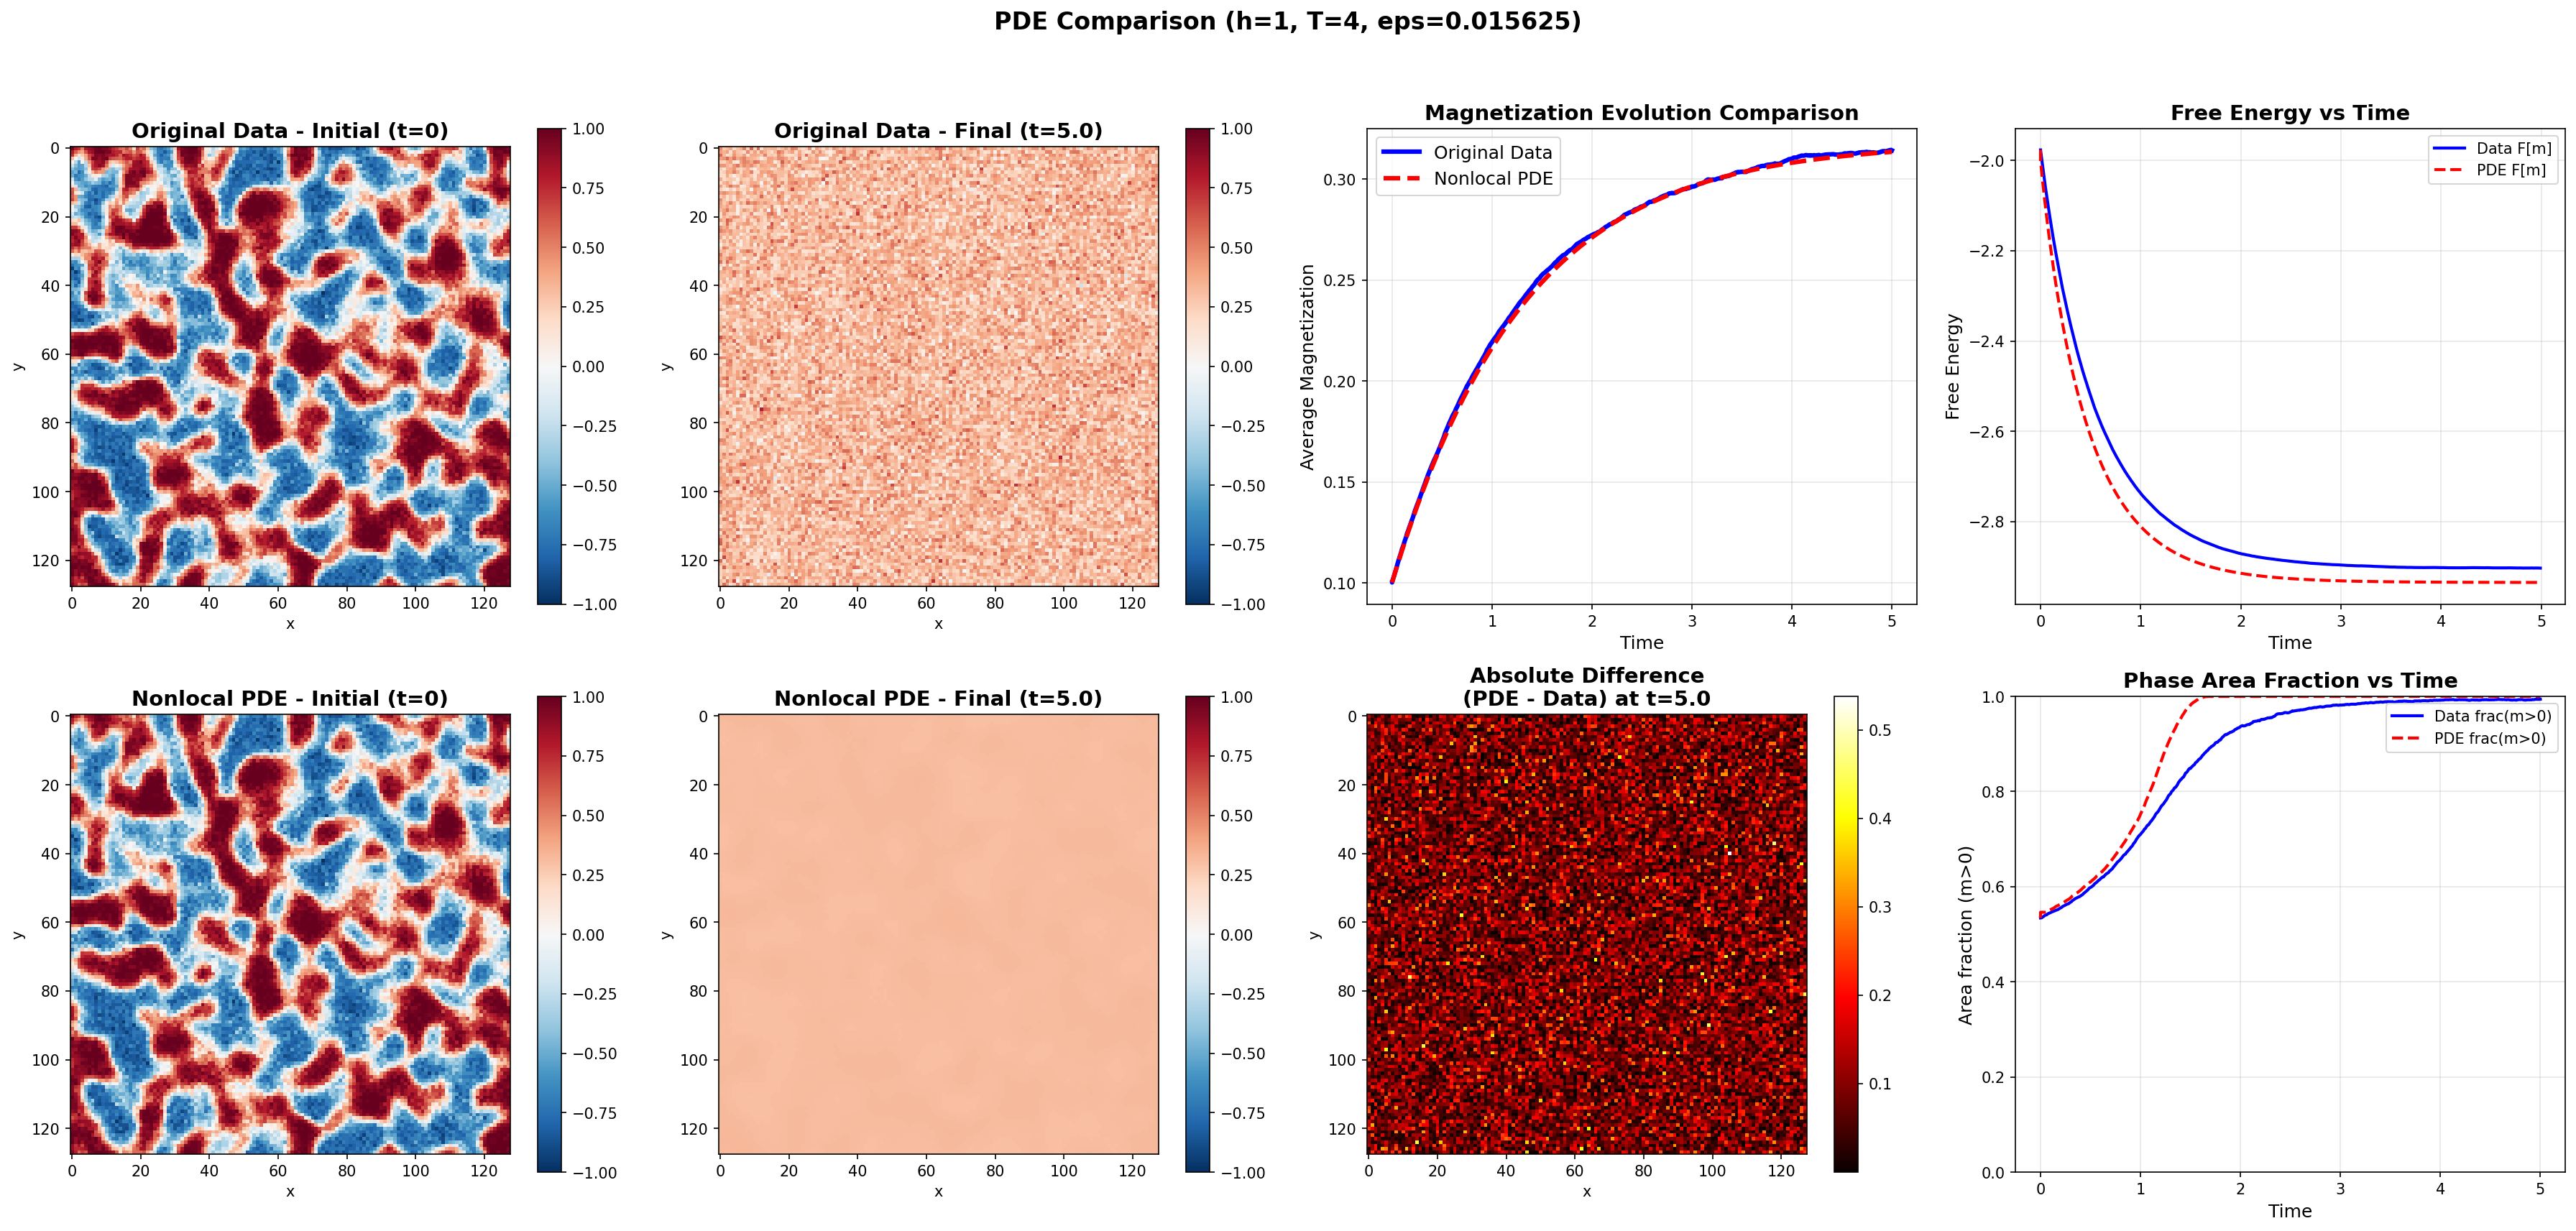
\includegraphics[width=1.0\textwidth]{fig/pde_comparison_h1_T4_eps0.015625.png}
    \caption{Comparison of original data and PDE solutions for $h=1$, $T=4$, $\epsilon=0.015625$.}
\end{figure}

% with epsilon = 0.03125

\begin{figure}[!h]
    \centering
    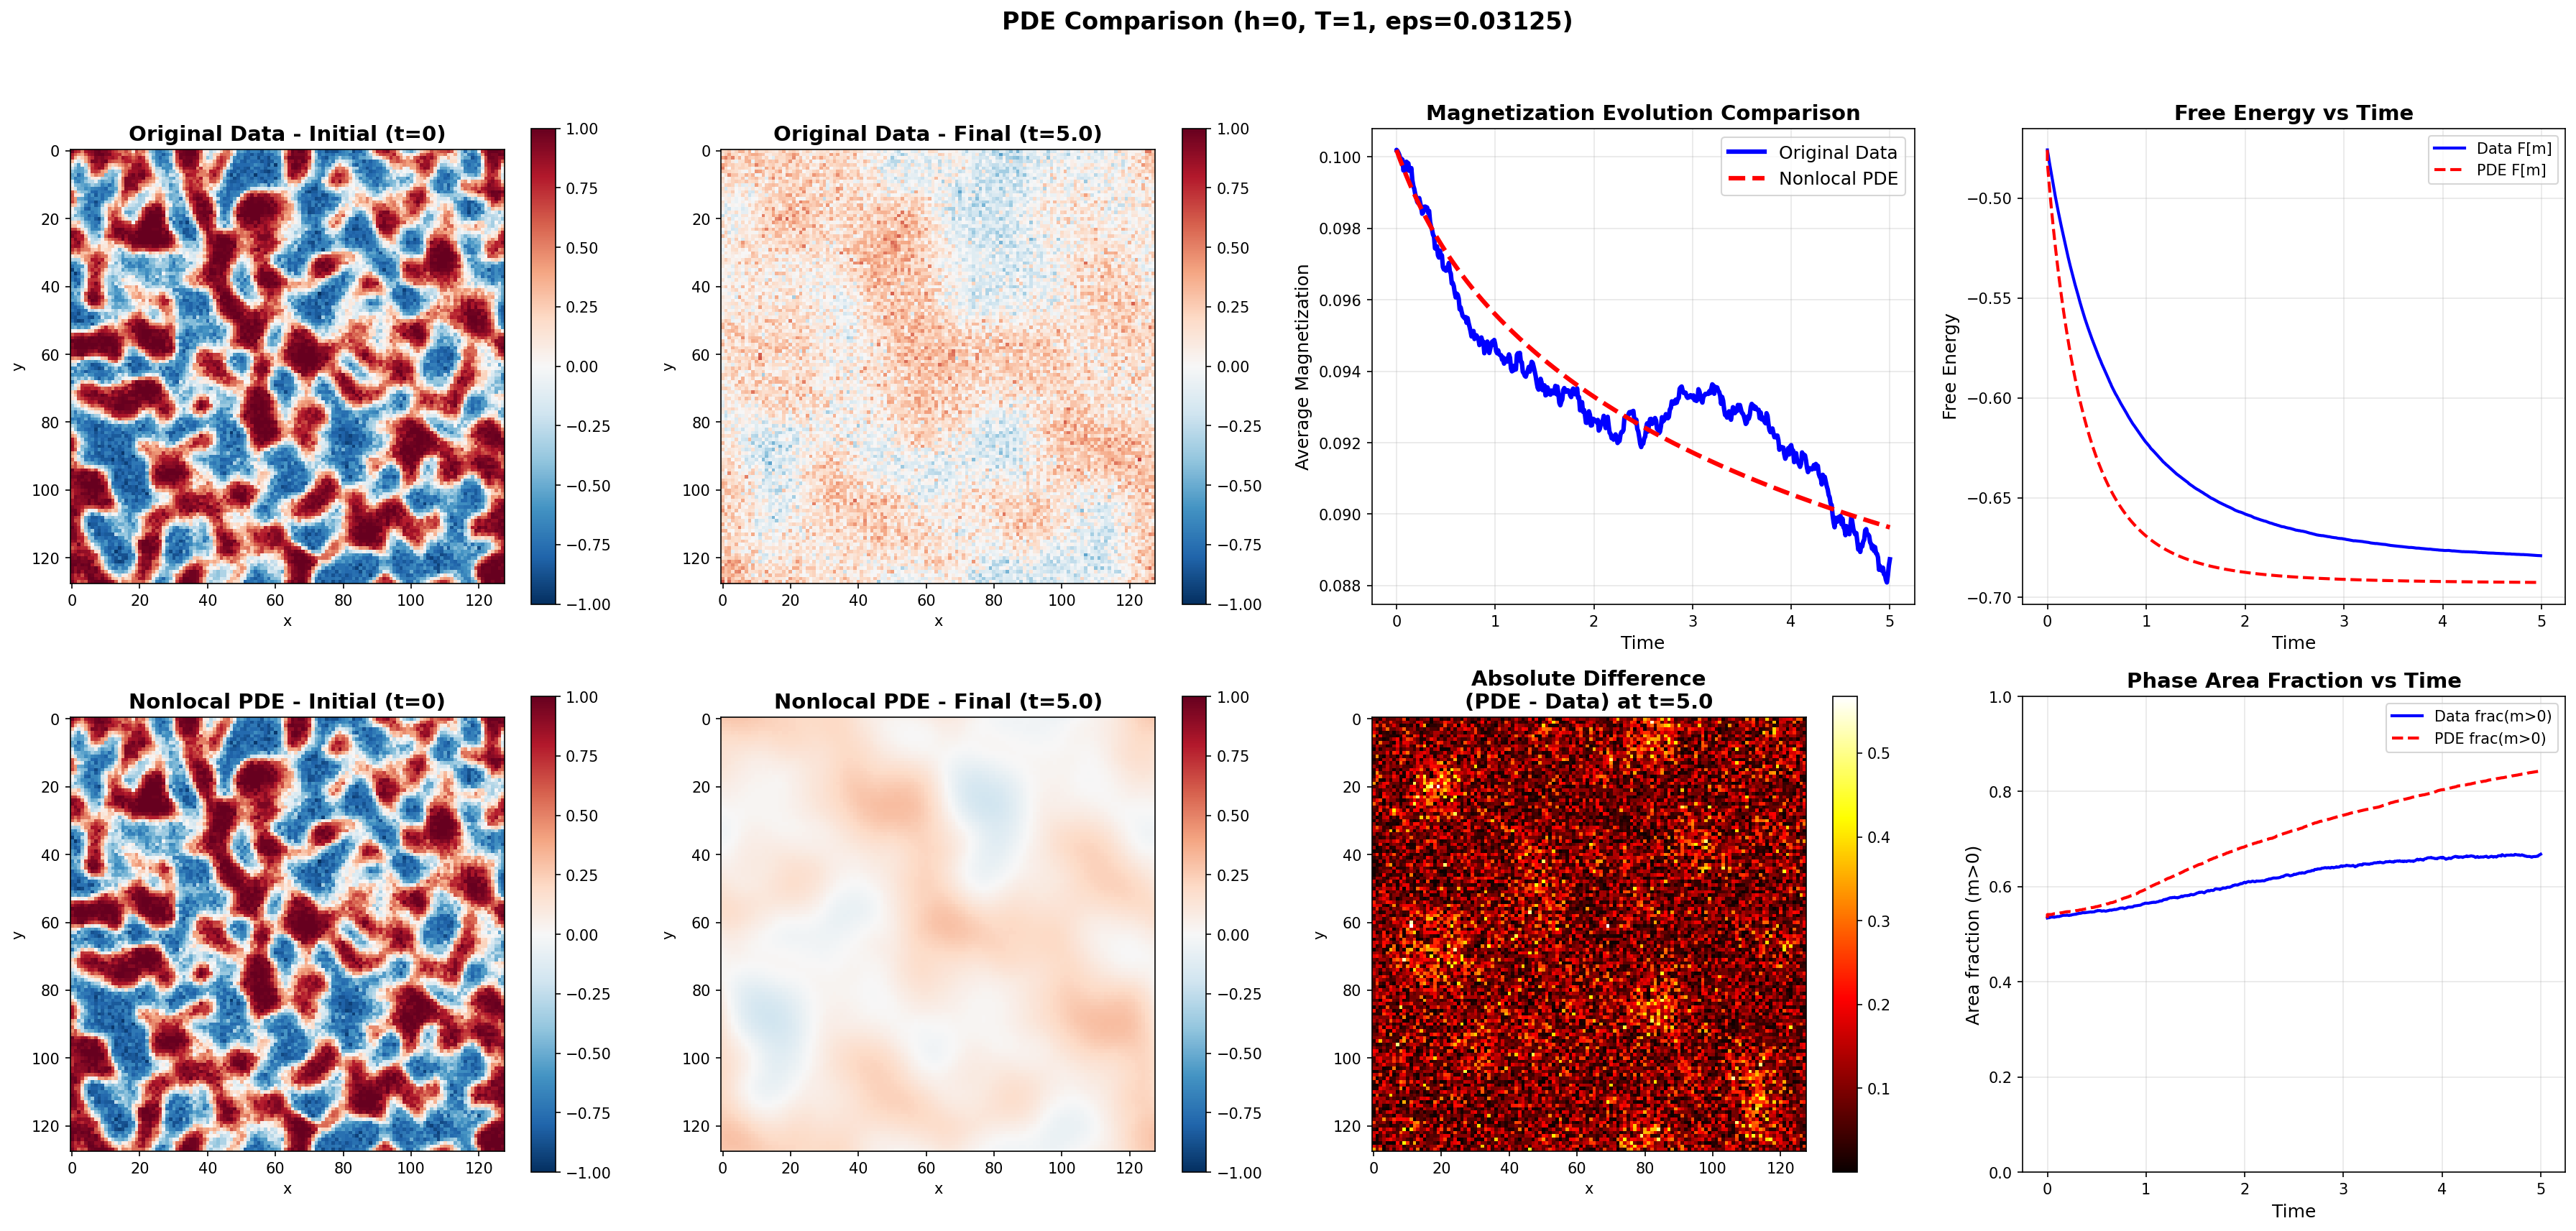
\includegraphics[width=1.0\textwidth]{fig/pde_comparison_h0_T1_eps0.03125.png}
    \caption{Comparison of original data and PDE solutions for $h=0$, $T=1$, $\epsilon=0.03125$.}
\end{figure}


\begin{figure}[h]
    \centering
    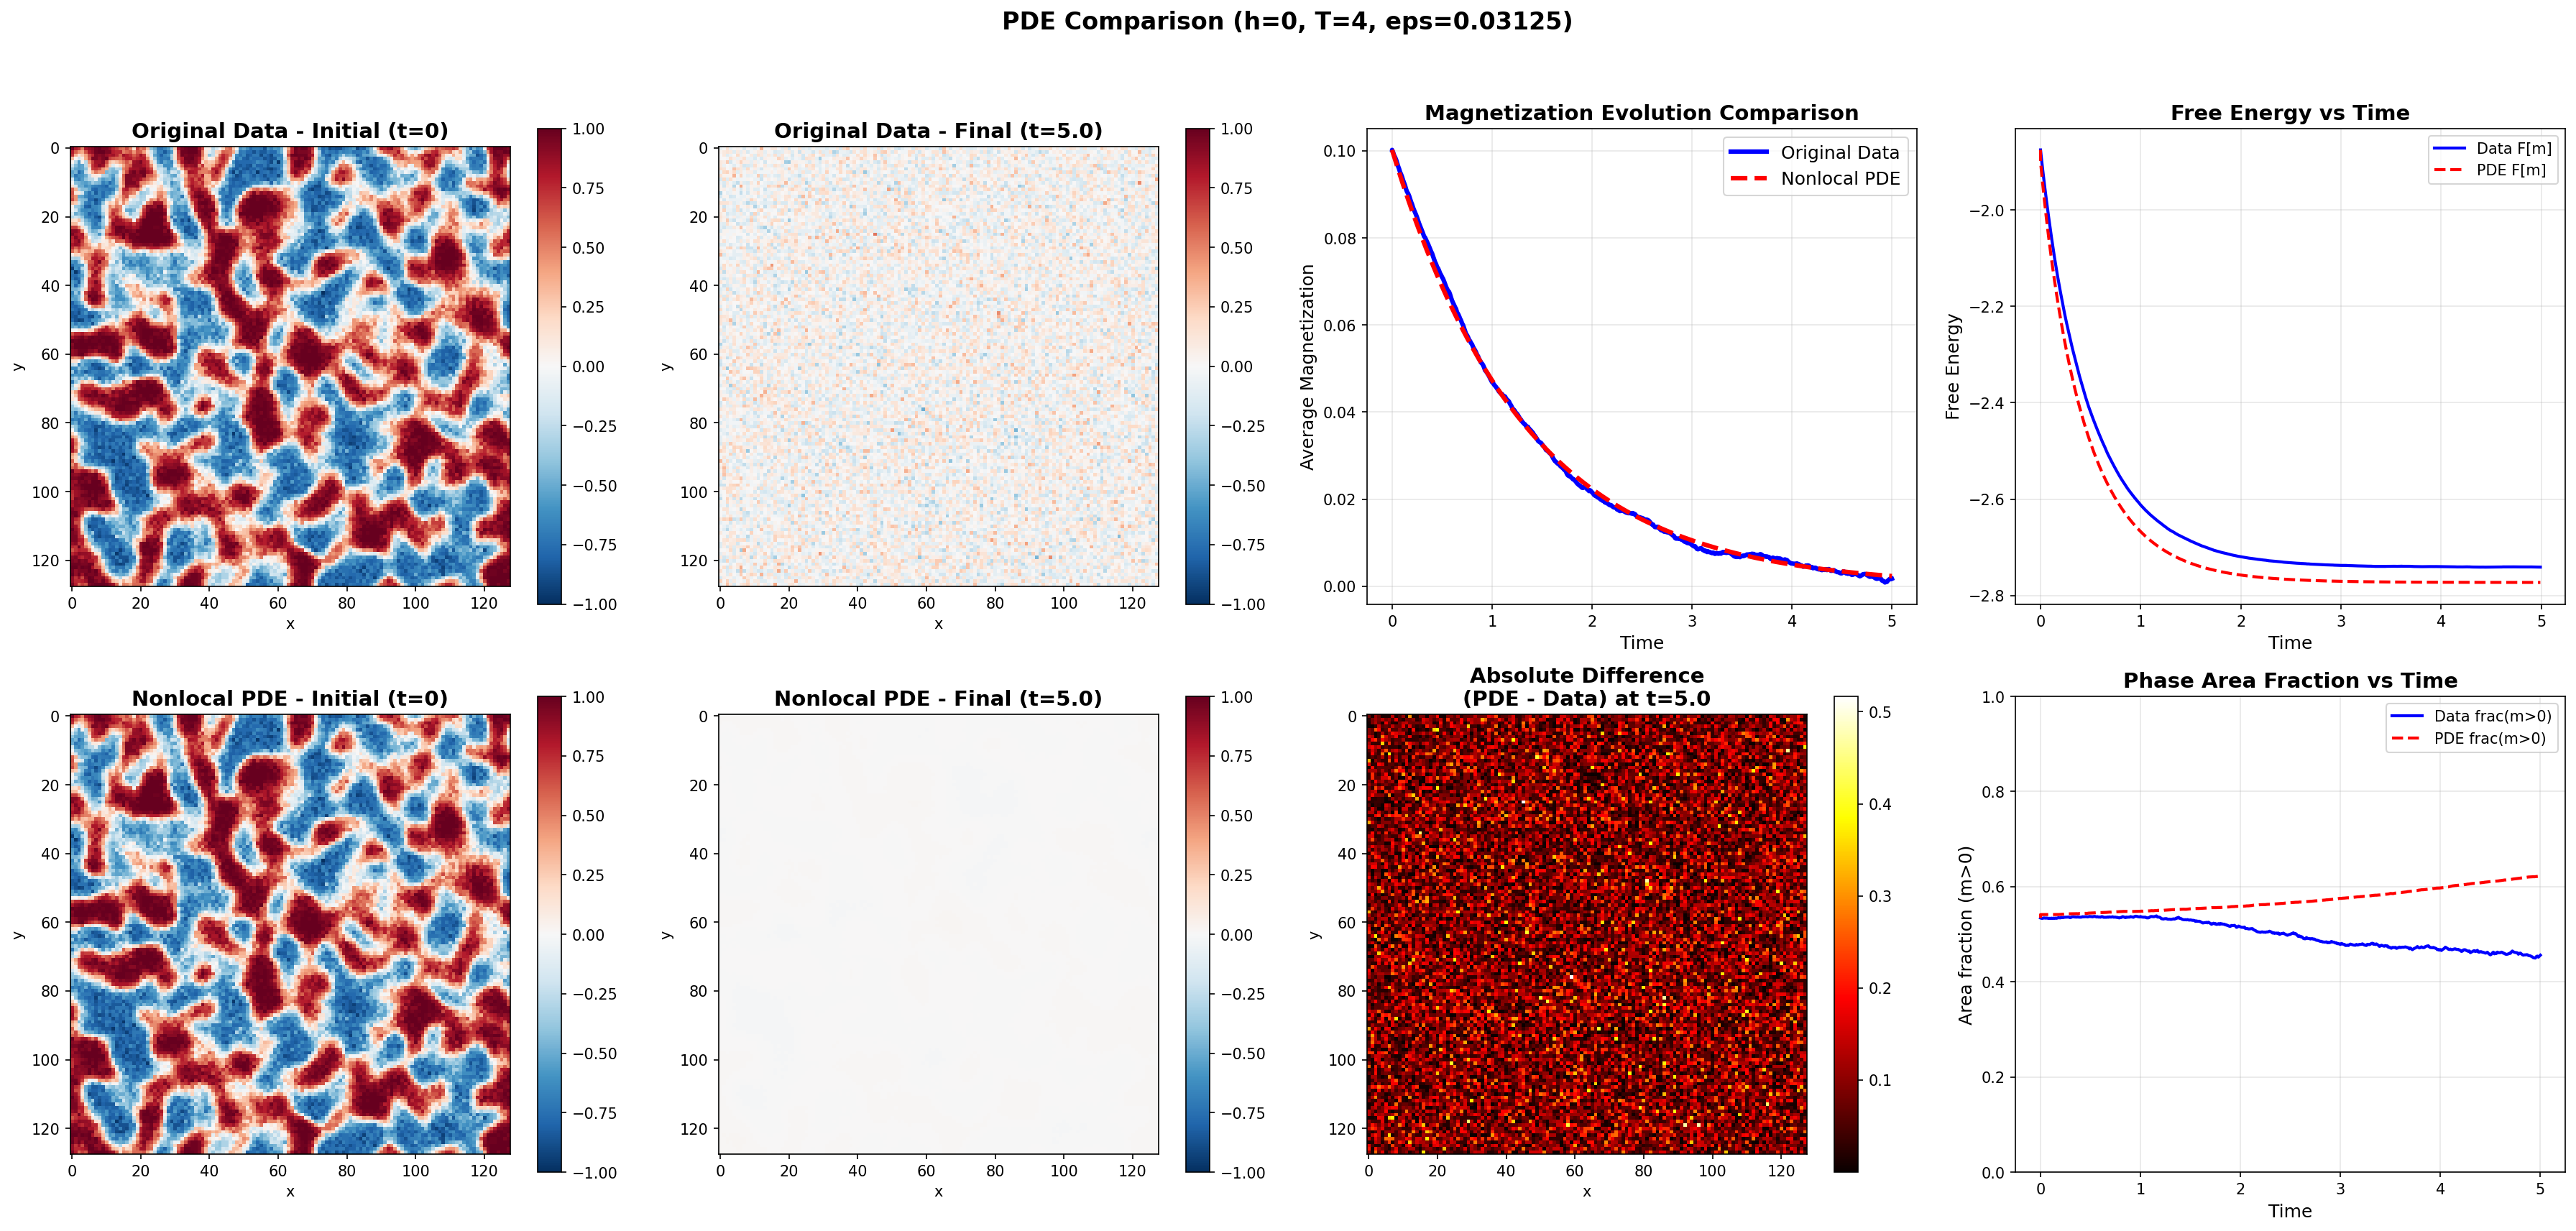
\includegraphics[width=1.0\textwidth]{fig/pde_comparison_h0_T4_eps0.03125.png}
    \caption{Comparison of original data and PDE solutions for $h=0$, $T=4$, $\epsilon=0.03125$.}
\end{figure}


\begin{figure}[!h]
    \centering
    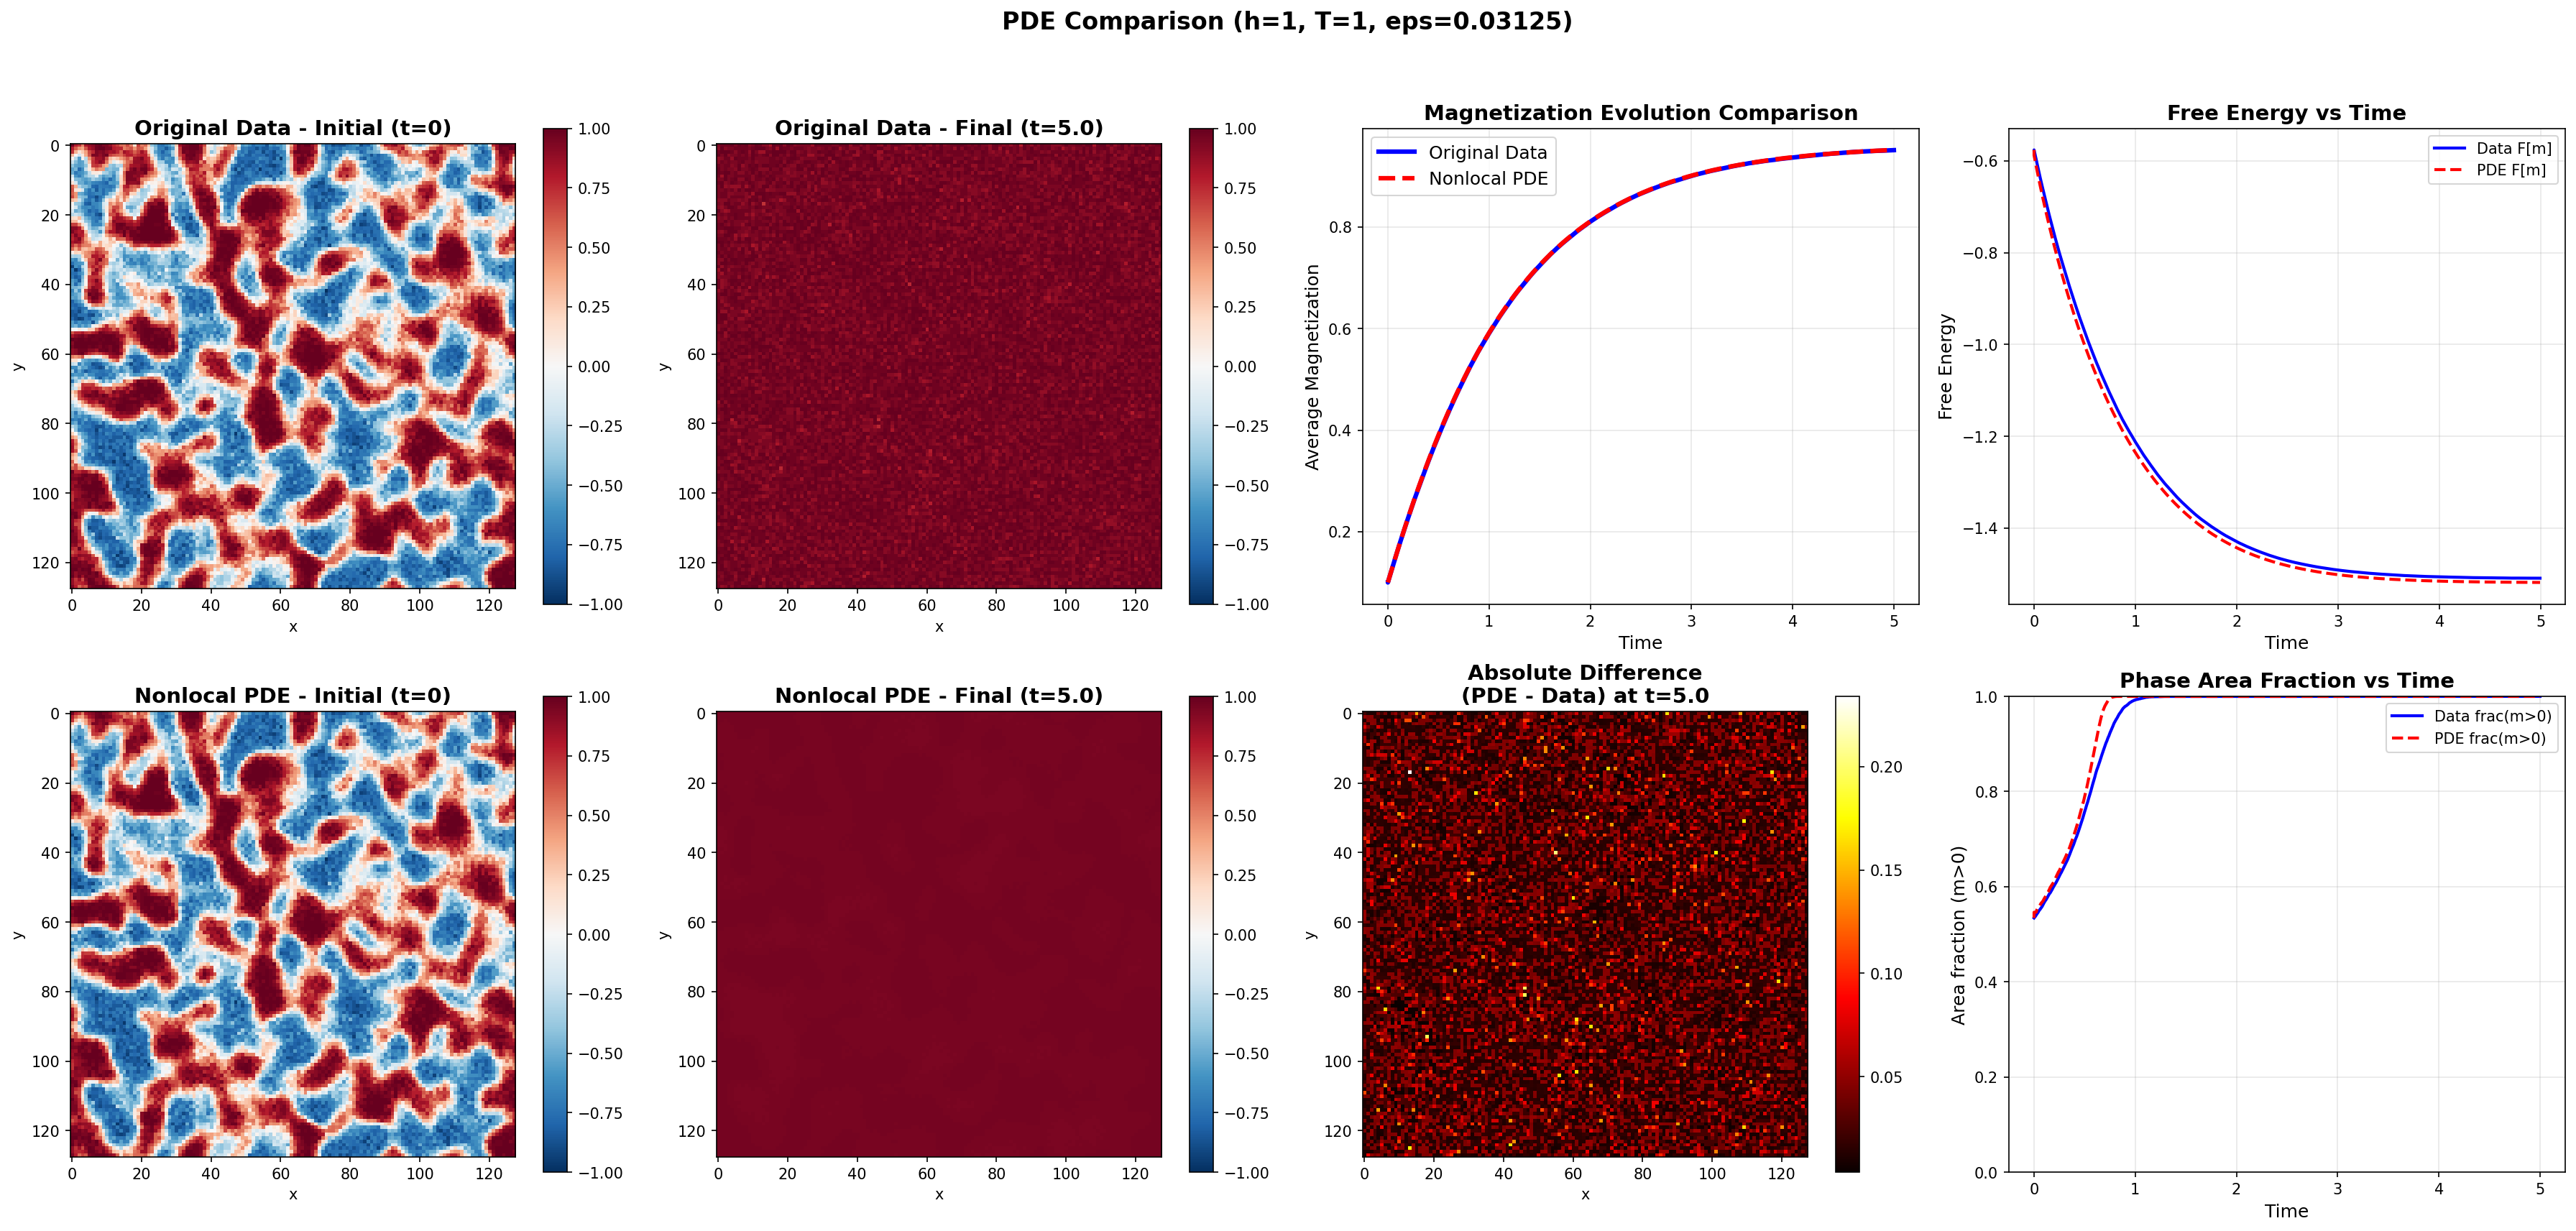
\includegraphics[width=1.0\textwidth]{fig/pde_comparison_h1_T1_eps0.03125.png}
    \caption{Comparison of original data and PDE solutions for $h=1$, $T=1$, $\epsilon=0.03125$.}
\end{figure}


\begin{figure}[h]
    \centering
    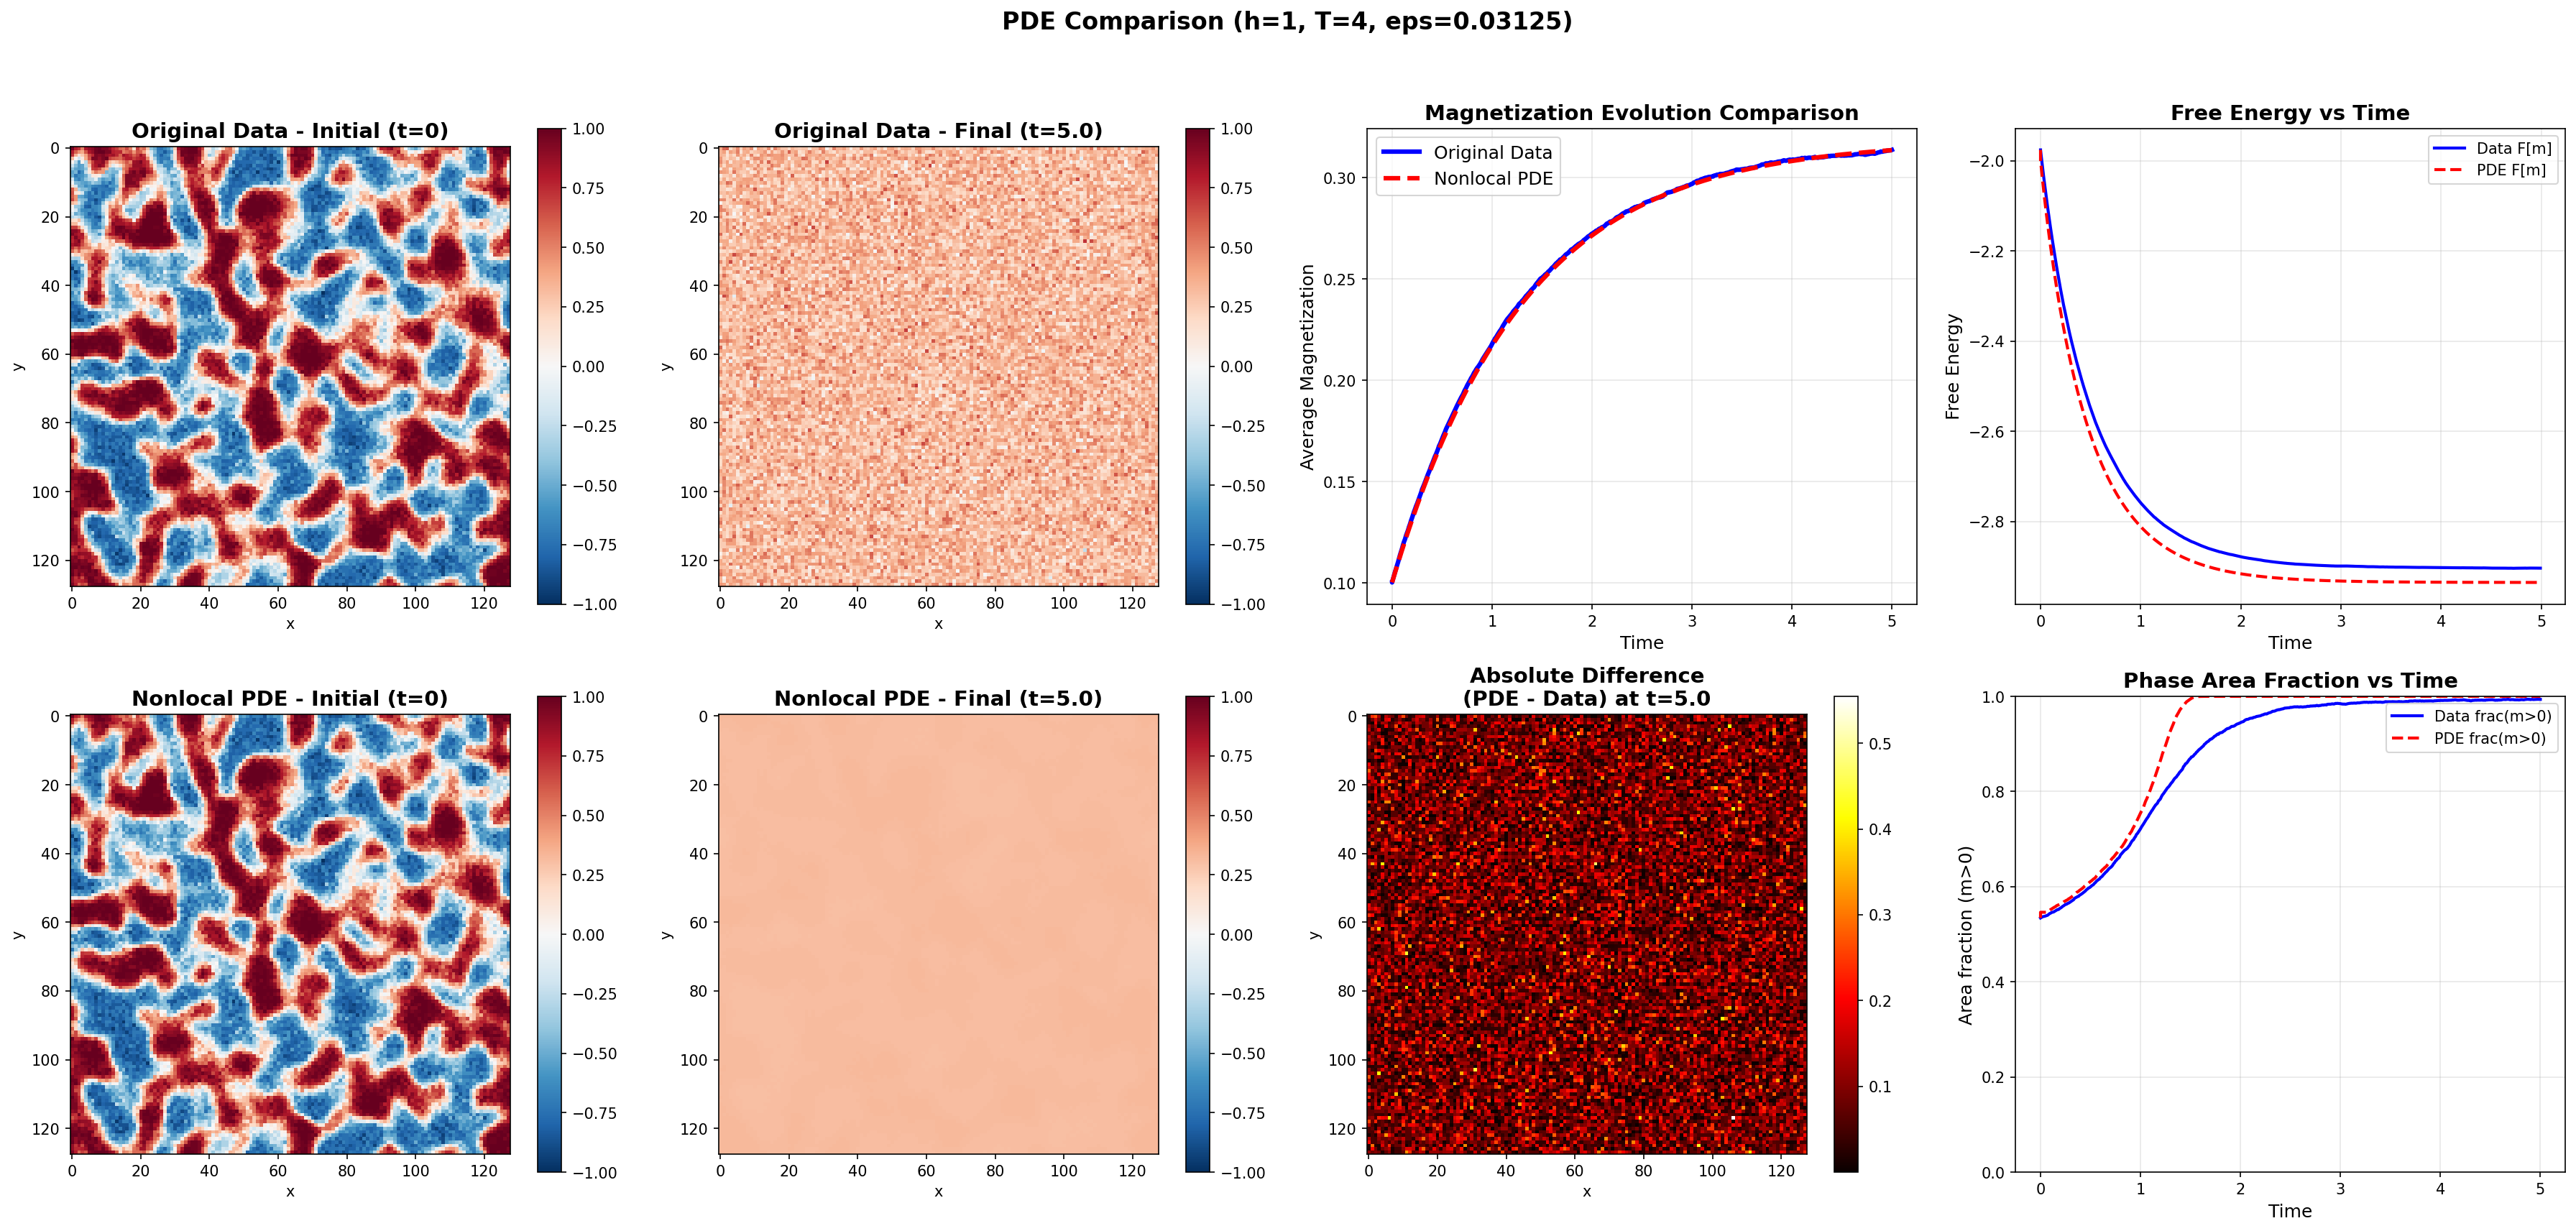
\includegraphics[width=1.0\textwidth]{fig/pde_comparison_h1_T4_eps0.03125.png}
    \caption{Comparison of original data and PDE solutions for $h=1$, $T=4$, $\epsilon=0.03125$.}
\end{figure}



\section{Network Training}

Recall that we want to train a network to predict the dynamics of the system.

\begin{equation}\label{eq:nonlocal-recall}
\partial_t m(t,x) \;=\; -\,m(t,x)\;+\;\tanh\!\Big(\beta\, (J_\gamma * m)(t,x) + \beta h\Big), \qquad m(0,x)=m_0(x),
\end{equation}



We have a generator parameterized like
\begin{equation}
    (\mathcal{L}m)(t,x) = F_\theta(I_\theta (m)(t,x), m(t,x))
\end{equation}

\begin{itemize}
    \item $m(.)$ can be a learned smooth function or $m_i$ itself; [-1, 1]
    \item $F_\theta(I,m)$ is $\mathbb{R}^2 \to \mathbb{R}$
    \begin{enumerate}
        \item Strong Prior: $F(I, m)=-Am+\tanh(\beta(BI+m+h))$; $F(I, m)=-Am+\tanh(BI+Cm+Dh))$, where $A,B,C,D$ are learnable parameters
        \item Weak Prior: an MLP with input size of 3 layers with hidden size of 128
    \end{enumerate}
    \item $I_\theta$ means we have a kernel $J_\theta$ to learn;
\end{itemize}


If the objective is to infer the interaction kernel J from data: 
(the obs part is obtained by difference? how we verify the learned structure?)

$$
J^\star, F^\star \;=\; \arg\min_{J, F}\;
\sum_{m \in \mathcal{D}}
\bigl\|\, \mathcal{L}(m;J,F)\;-\;\partial_t m_{\mathrm{obs}} \,\bigr\|_{L^2(\Omega)}^{2}.
$$


\end{document}